\section{Introduction}

\begin{figure*}

  \begin{panel}{(a)}{\textwidth}
    \vspace{5mm}
    \small
    \tikzsetnextfilename{figure_1_overview}
    \usetikzlibrary{spy}%
\def\blinky#1#2#3#4#5{%
  \begin{tikzpicture}[node distance=3mm]
    \node[site#1] (s1) {};
    \node[site#2,right of=s1] (s2) {};
    \coordinate (s12) at ($(s1)!.5!(s2)$);
    \node[site#3,right of=s2] (s3) {};
    \node[site#4,below of=s12] (s4) {};
    \node[site#5,right of=s4] (s5) {};
    \foreach \angle in {0, 45, 90, 135, 180, 225, 270, 315}{
      \begin{scope}[rotate=\angle]
        \draw[sitelight#1] ($(s1)+(0,0.13)$) -- ($(s1)+(0,0.16)$);
        \draw[sitelight#2] ($(s2)+(0,0.13)$) -- ($(s2)+(0,0.16)$);
        \draw[sitelight#3] ($(s3)+(0,0.13)$) -- ($(s3)+(0,0.16)$);
        \draw[sitelight#4] ($(s4)+(0,0.13)$) -- ($(s4)+(0,0.16)$);
        \draw[sitelight#5] ($(s5)+(0,0.13)$) -- ($(s5)+(0,0.16)$);
      \end{scope}
    }
  \end{tikzpicture}
}%
\begin{tikzpicture}

  \begin{scope}[spy using outlines={magnification=2,size=12mm,very thick}]

    \node[image] (frame) {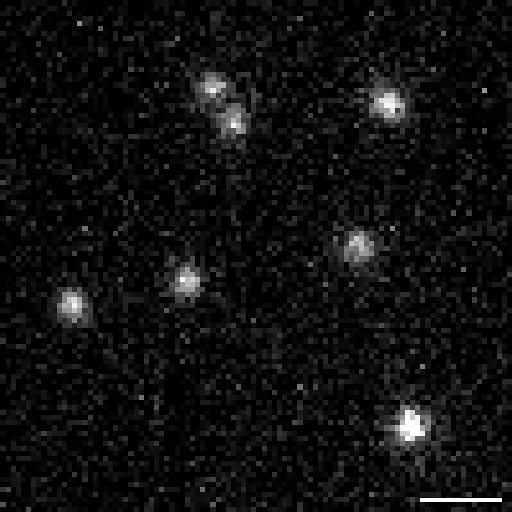
\includegraphics[width=4cm]{figures/data/overview/sample_frame}};

    \spy on ($(frame)+(1.1, 1.2)$)
      in node (patch_3) [image,right=6mm,anchor=north west]
      at (frame.north east);
    \spy on ($(frame)+(0.9, 1.1)$)
      in node (patch_2) [image,right=6mm,anchor=north west]
      at ($(frame.north east)-(0.1,0.1)$);
    \spy[
        draw=funkey_color_1,
        every spy on node/.append style={ultra thick},
        every spy in node/.append style={ultra thick},
        spy connection path={\draw[ultra thick] (tikzspyonnode) -- (tikzspyinnode);}
    ]
      on ($(frame)+(1.0, 1.2)$)
      in node (patch_1) [image,right=6mm,anchor=north west]
      at ($(frame.north east)-(0.2,0.2)$);
  \end{scope}

  % example trace
  \node[right=4mm,anchor=north west,text width=6cm,inner sep=0] (trace) at (patch_3.north east) {%
    \def\tracecsv{figures/data/overview/trace.csv}%
    \def\traceintensitycol{trace}%
    \def\nolabels{}%
    \tikzexternaldisable%
    \centerline{\begin{tikzpicture}%
  \begin{axis}[
    name=trace,
    width=0.8\textwidth,
    height=5cm,
    xlabel=frames,
    ylabel=intensity,
    enlarge x limits=false,
    xtick distance=500,
    grid=major,
    grid style={dashed},
    scaled ticks=false,
    ticklabel style={font=\small},
    legend style={nodes={scale=0.6, transform shape}},
  ]

    \addplot [
      color=tracecolor,
      mark=*,
      mark size=0.7pt,
      mark options={line width=0},
      fill opacity=0.8,
      draw opacity=0.2,
    ] table [
      col sep=comma,
      x=frames,
      y=\traceintensitycol
    ] {\tracecsv};
    \addlegendentry{intensity trace}

    \addplot [
      color=ztracecolor,
      thick
    ] table [
      col sep=comma,
      x=frames,
      y=\zcol
    ] {\tracecsv};
    \addlegendentry{inferred state}

    % remember min/max y-axis values for next plot
    \pgfplotsextra{
      \pgfmathparse{\pgfkeysvalueof{/pgfplots/ymin}}
      \global\let\ymin\pgfmathresult
      \pgfmathparse{\pgfkeysvalueof{/pgfplots/ymax}}
      \global\let\ymax\pgfmathresult
    }

  \end{axis}

  \begin{axis}[
    at={($(trace.east) + (4mm,0)$)},
    anchor=west,
    width=0.3\textwidth,
    height=5cm,
    yticklabel=\empty,
    xtick distance=0.005,
    xlabel=probability,
    grid=major,
    grid style={dashed, very thin},
    enlarge x limits={value=0.1,upper},
    scaled ticks=false,
    ymin=\ymin,
    ymax=\ymax,
    ticklabel style={font=\small},
    legend style={nodes={scale=0.6, transform shape}},
  ]

    \addplot+[
      xbar interval,
      mark=none,
      color=tracecolor,
      fill=tracecolor,
      fill opacity=0.6,
      draw=none,
    ] table [
      col sep=comma,
      y=\histbincol,
      x=\histcountcol,
    ] {\histogramcsv};
    \addlegendentry{intensity histogram}

    \addplot[
      color=intensitymodelcolor!80!black,
      thick
    ] table [
      col sep=comma,
      y=\histbincol,
      x=\modelfitcol
    ] {\histogramcsv};
    \addlegendentry{inferred model}

  \end{axis}
\end{tikzpicture}%
}%
    \tikzexternalenable%
  };
  \node[anchor=north,inner sep=0pt] at (trace.230) {\tiny time};
  \node[rotate=90,anchor=south,inner sep=1pt] at (trace.west) {\tiny intensity};

  % observed / hidden line
  \draw[gray,very thick]
    (patch_1.west|-frame.355) --
      node[pos=0,anchor=south west] {observed}
      node[pos=0,anchor=north west] {hidden}
      node[pos=0.35] (sample_1) {}
      node[pos=0.60] (sample_2) {}
      node[pos=0.96] (sample_3) {}
    (trace.east|-frame.355);

  % brace to MLE
  \draw[decorate,decoration={brace,raise=2mm}]
    (trace.north east) --
    node[pos=0.5,right=5mm,draw,rectangle,rounded corners] (mle) {\ours}
    (trace.south east);

  % posterior
  \node[anchor=north west,text width=3.6cm] (posterior) at ($(trace.north east)+(1.8,0.3)$) {%
    \def\posteriorcsv{figures/data/overview/posterior.csv}%
    \def\posteriorcol{posterior}%
    \def\noylabels{}%
    \tikzexternaldisable%
    \@ifundefined{noylabels}{}{%
  \pgfplotsset{yticklabel=\empty}%
}%
\begin{tikzpicture}%

  \def\eps{0.001}

  \begin{axis}[
    width=\textwidth,
    height=\textwidth,
    xlabel=\n,
    xlabel=$p(\n|\trace)$,
    grid=major,
    grid style={dashed, very thin},
    enlarge x limits=0.1,
    enlarge y limits=0,
    ymin=0,
    ymax=1,
    scaled ticks=false,
    ticklabel style={font=\small},
  ]

    \addplot+[
      ybar,
      bar width=1,
      mark=none,
      fill=posteriorcolor,
      fill opacity=0.6,
      draw=posteriorcolor,
      y filter/.expression={
        y < \eps ? nan : y
      },
    ] table [
      col sep=comma,
      y=\posteriorcol,
      x=n,
    ] {\posteriorcsv};

    \ifdefined\posteriorcolextra
      \addplot+[
        ybar,
        bar width=1,
        mark=none,
        fill=posteriorcolor!60!black,
        fill opacity=0.6,
        draw=posteriorcolor,
        y filter/.expression={
          y < \eps ? nan : y
        },
      ] table [
        col sep=comma,
        y=\posteriorcolextra,
        x=n,
      ] {\posteriorcsv};
    \fi

  \end{axis}

\end{tikzpicture}
%
    \tikzexternalenable%
  };
  \draw[arrow,shorten >=-8] (mle) -- (mle-|posterior.west);

  % blinky things
  \node (hidden) at (frame.330-|patch_1) {\blinky{off}{off}{off}{off}{off}};
  \node (z_sample_1) at (frame.330-|sample_1) {\blinky{on}{off}{on}{on}{off}};
  \node (z_sample_2) at (frame.330-|sample_2) {\blinky{on}{off}{on}{off}{off}};
  \node (z_sample_3) at (frame.330-|sample_3) {\blinky{on}{off}{off}{off}{off}};

  \draw[arrow] (z_sample_1) -- +(0, 2.4);
  \draw[arrow] (z_sample_2) -- +(0, 2.05);
  \draw[arrow] (z_sample_3) -- +(0, 1.7);

  \node[anchor=north,inner sep=10pt] at (hidden) {\strut$\n=5$};
  \node[anchor=north,inner sep=10pt] at (z_sample_1) {\strut$\z{}=3$};
  \node[anchor=north,inner sep=10pt] at (z_sample_2) {\strut$\z{}=2$};
  \node[anchor=north,inner sep=10pt] at (z_sample_3) {\strut$\z{}=1$};

\end{tikzpicture}

    \vspace{-2mm}
  \end{panel}

  \begin{panel}{(b)}{0.6\textwidth}
    \begin{panel}{}{\textwidth}
      \small
      \tikzsetnextfilename{figure_1_p_on_off}
      \centerline{\begin{tikzpicture}
  \node[siteoff,inner sep=4pt] (off) {};
  \node[siteon,right=2cm of off,inner sep=4pt] (on) {};
  \foreach \angle in {0, 45, 90, 135, 180, 225, 270, 315}{
    \begin{scope}[rotate=\angle]
      \draw[sitelighton,ultra thick] ($(on)+(0,0.26)$) -- ($(on)+(0,0.32)$);
    \end{scope}
  }
  \draw[arrow,shorten >=2mm,shorten <=2mm] (off) to[bend left] node[pos=0.5,above] (pon) {\pon} (on);
  \draw[arrow,shorten >=2mm,shorten <=2mm] (on) to[bend left] node[pos=0.5,below] {\poff} (off);

  \node[right=14mm of on] (re) {$\sim\poisson(\re\deltat)$};
  \draw[arrow,decorate,decoration={coil,aspect=0,segment length=6,post=curveto,post length=2mm}] ($(on.east)+(0.2,0)$) -- (re);

  %\node[parameters,anchor=south] at (re.north) {\strut$\parameterst = (\pon, \poff)$};

  \node[above=1mm of pon,gray] {transition model};
\end{tikzpicture}
}
    \end{panel}

    \vspace{4mm}
    \begin{panel}{(c)}{\textwidth}
      \small
      \hspace{4mm}
      \tikzsetnextfilename{figure_1_intensity_model}
      \begin{tikzpicture}

  \node (z) {\blinky{on}{off}{on}{on}{off}};
  \node[var,right=18mm of z] (c) {$\photons$};
  \node[annotation,below of=c] (c_dist) {$\sim\poisson((\z{}\re + \rb)\deltat)$};
  \draw (c) -- (c_dist);
  \draw[arrow,decorate,decoration={coil,aspect=0,segment length=6,post=curveto,post length=3mm}]
    (z.east) -- (c);

  \node[right=12mm of c,inner sep=0,yshift=2mm] (camera) {
    \tikz[plane x={(0.8,-0.4)},canvas is plane,transform shape]{
      \draw[gray,step=0.25] (0, 0) grid (1, 1);
      \node[anchor=south,gray] at (0.5, 1.1) {detector};
    }
  };

  \coordinate (camera_center) at (camera.center|-c);
  \draw[arrow,shorten >=3mm] (c) -- (camera_center);
  \node[observation,right=18mm of camera_center] (x) {$\x{}$};
  \node[annotation,below of=x] (x_dist) {$\sim\mathcal{N}(\photons\camgain + \camoffset, \camvar)$};
  \draw (x) -- (x_dist);
  \draw[arrow] (camera.east|-c) -- (x);
  \node[below=1mm of z] {\z{}};

  % parameter collections
  %\node[parameters,anchor=south west] at (z.north east) {\strut$\parameterse = (\re, \rb)$};
  %\node[parameters,anchor=south east] at (z.north-|x_dist.east) {\strut$\parametersc = (\camgain, \camoffset, \camvar)$};

  % annotations
  \node[above=2mm of c,gray] {\strut emission model};
  \node[above=2mm of x,gray] {\strut camera model};
\end{tikzpicture}

    \end{panel}
  \end{panel}
  \begin{panel}{(d)}{0.35\textwidth}
    \small
    \vspace{4mm}
    \hspace{4mm}
    \tikzsetnextfilename{figure_1_model}
    \centerline{\begin{tikzpicture}

  % parameters
  \node[var] (n) {\n};
  \node[var,below of=n] (theta_T) {\parameterst};
  \node[var,below of=theta_T] (theta_E) {\parameterse};
  \node[var,below of=theta_E] (theta_C) {\parametersc};

  % hidden states
  \node[state,right=1cm] (z1) at ($(n)!.5!(theta_T)$) {\z{1}};
  \node[state,right=4mm of z1] (z2) {\z{2}};
  \node[state,right=1cm of z2] (zt) {\z{t}};
  \node at ($(z2)!.5!(zt)$) {$\cdots$};

  % observations
  \node[observation,right=1cm] (x1) at ($(theta_E)!.5!(theta_C)$) {\x{1}};
  \node[observation,right=4mm of x1] (x2) {\x{2}};
  \node[observation,right=1cm of x2] (xt) {\x{t}};
  \node at ($(x2)!.5!(xt)$) {$\cdots$};

  % plates
  \begin{pgfonlayer}{background}
    \node[plate,fit=(z1)(zt)] (hidden) {};
    \node[plate,fit=(x1)(xt)] (observed) {};
  \end{pgfonlayer}

  % dependencies
  \draw[arrow] (n) to (hidden);
  \draw[arrow] (theta_T) to (hidden);
  \draw[arrow] (theta_E) to (observed);
  \draw[arrow] (theta_C) to (observed);
  \draw[arrow] (z1) to (x1);
  \draw[arrow] (z2) to (x2);
  \draw[arrow] (zt) to (xt);
  \draw[arrow] (z1) to (z2);
  \draw[arrow,shorten <=20] (z2) to (zt);
  \draw[shorten >=22] (z2) to (zt);

  % annotation
  \node[below of=observed] {$p(\trace|\n,\parameterst,\parameterse,\parametersc)$};

\end{tikzpicture}
}
  \end{panel}

  \caption{
      \panelref{a} Overview of the blinx method (scale bar: 1 $\mu$m)
      %
      \panelref{b} TODO
      %
      \panelref{c} TODO
      %
      \panelref{d} TODO \ours is based on a Hidden Markov Model who's
      parameters are optimized to build the final posterior distribution
  }
  \label{fig:method:overview}
\end{figure*}


% molecular counting: what is it and why do we care?
%
Molecular counting aims to determine the absolute number of \smallobjects
associated in an \object, a quantity that is often essential to understanding
the underlying biology of a system.
  %
  The activation of T cells, for example, is sensitive to single ligands, and
  quantifying the molecular count of ligand-receptor interactions informs
  understanding of downstream signalling pathways and
  sensitivity~\citep{irvine_2002}.
  %
  Furthermore, molecular counting allows identifying oligomeric states by
  counting the subunits in a cluster, to tell monomers, dimers,
  trimers, and higher order oligomers apart.
  %
  Several biological processes depend on this quantity: TGF-$\beta$ signaling,
  for example, depends on the oligomeric state of Smad~\citep{inman_2002,
  moustakas_2002}.
  %
  Similarly, the oligomeric state of G-protein coupled receptors influences
  downstream GPCR signaling~\citep{felce_2018, breitwieser_2004}.

% fluorescence microscopy alone is not enough
%
Often, as in those examples, the \smallobjects of interest are only a few
nanometers apart and as such can not be quantified in standard fluorescence
microscopy.
  %
  %Fluorescence microscopy can provide precise localization information of
  %molecular species, but its ability to determine quantitative information, such
  %as counts of nearby molecules, remains limited.
  %
  In contrast to larger structures (whole cells or organelles), which can
  easily be discerned in fluorescence microscopy, individual molecules in
  diffraction limited spots below a resolution of 200\nanometer can no longer
  be separated.
  %
  Even super-resolution techniques~\citep{betzig_2006,rust_2006} that surpass
  the diffraction limit are not suitable to discern \smallobjects that are
  closer than 10\nanometer apart~\citep{valli_seeing_2021}.
  %
  However, many \objects of interest are smaller still, or physically
  positioned closer together and cannot be spatially separated even with
  super-resolution techniques.
  %\todo{other reasons why super resolution is not always possible/desirable? imaging speed?}
  % ^^ any limitations to super-res will also effect our method

% summary of what the problem is and how we approach it
%
We present a Bayesian solution to estimate the number of fluorescently labelled
\smallobjects in a single diffraction limited spot.
  %
  Our solution is based on a probabilistic model that incorporates the
  photo-physics of blinking fluorescent emitters and models their dynamics over
  time as a Markov chain.
  %
  Given a trace of the combined intensity of all \smallobjects contained in a
  spot over time, this model can be used to obtain a posterior distribution
  over the number of emitters contained in that spot.

% Motivate fluorescence based methods (doesn't say a lot IMO -Jan)
%
%
%Although other methods exist to quantify molecular count at this scale, a
%robust, accurate, \todo{needs citations} fluorescence based method would make
%quantification much more accessible, while maintaining the benefits of
%fluorescence imaging, such as spatial localization.

%%%%%%%%%%%%%%%%
% Related Work %
%%%%%%%%%%%%%%%%

% fluorescence intensity based counting
%
Perhaps the simplest method of molecular counting is to correlate the combined
fluorescent intensity of a spot with the number of \smallobjects, \ie, the
brighter the spot is, the more \smallobjects are contained~\citep{schmied_2012,
tolar_2005}.
  %
  This method works well for qualitative measures, but, due to the noise in
  intensities measured from any single fluorophore, lacks the precision needed
  to report exact counts.

% Other methods work by separating things out in time
%
Molecular counting can be more reliable if temporal fluctuations of intensity
are observed.
  %
  % FCS and bSOFI
  Methods such as fluorescence correlation spectroscopy
  (FCS)~\citep{otsuka_2023,wachsmuth_2015,politi_2018} and balanced
  super-resolution optical fluctuation imaging
  (bSOFI)~\citep{geissbuehler_2012} fit higher order statistics to fluctuations
  in fluorescent intensity over time to estimate the molecular count.
  % Bleaching based
  In other methods, temporal variations in intensity are induced rather than
  just observed, \eg, by measuring the number of distinct bleaching
  steps that provide cues about the number of fluorescent
  emitters~\citep{ulbrich_2007,jain_2011,hummert_2021}.

% Some of those use blinking fluorophores
%
Blinking fluorophores, such as those used in
PALM~\citep{sengupta_pcPALM_2011,lee_counting_2012} and
STORM~\citep{patel_blinking_2021}, can be used to facilitate the counting
problem~\citep{rollins_stochastic_2015,nino_2017}.
  %
  % Some of these methods are also based on HMMs, should we mention that here?
  The known blinking behavior allows for more precise models than the random
  fluctuations measured in FCS and bSOFI, while the repeated transitions in
  intensity provide more information than the irreversible switch in bleaching
  based counting.
  %
  % Limitations
  A major limitation of these methods is the effect of photo-bleaching, as this
  limits the amount of time a single fluorophore can be observed, and makes it
  difficult to differentiate blinking from photo-bleaching.

% DNA-PAINT is extra useful because its emitters dont bleach either
%
In contrast, DNA-PAINT~\citep{schnitzbauer_2017} is a method of producing
blinking fluorescence that is functionally immune to photo-bleaching due to the
continuous replenishment of fluorophores from solution~\citep{stehr_2021}.
  %
  % lbFCS
  Localization based FCS (\lbfcs)~\citep{stein_2019,stein_2021} combines the
  structured blinking of DNA-PAINT with the principles of FCS, fitting the
  autocorrelation function of intensity over time to produce a count. As such,
  it is able to accurately count up to six molecules in a single diffraction
  limited spot.
  %
  % qPAINT
  Quantitative DNA-PAINT (qPAINT~\citep{jungmann_2016}) estimates the molecular
  count based on the frequency of blinking events, \ie, a blinking rate of one
  event per second is calibrated to one molecule, therefore an observation of
  ten events per second produces a count of ten molecules.
  % Limitations
  However, both of these methods are limited in that they fit summary
  statistics, rather than the data directly.
  %
  In contrast, our solution fits the model to each frame of the measurement 
  in sequence, fully utilizing both the temporal and intensity information available.
  %
  Further, all of the methods mentioned provide a single estimate of molecular count. 
  %
  A probabilistic estimate would identify cases where different possible counts are all likely,
  as well as provide a measure of certainty in the count. Providing a more detailed quantitative 
  understanding of the system. 

% Our Model
% ----------
% fully Bayesian
We propose \ours, a fully Bayesian model to estimate the molecular count
directly from a fluctuating sequence of fluorescent intensity measurements over
time.
  %
  % Based on a fully differentiable markov chain
  Based on a fully differentiable Hidden Markov Model, \ours fits
  seven parameters (blinking on/off rates, emitter and background photon emission rates, 
  and camera gain/offset/variance) directly to the sequence of measurements, 
  estimating a likelihood for each possible count.
  % probabilistic
  These likelihoods can be directly compared, producing a posterior
  distribution of counts given the observation sequence.
  % more accurate than existing methods 
  We validated \ours on a series of simulated experiments, and shows a
  significant improvement in performance over both \lbfcs and \qpaint.
  %
  Finally, we proved the counting ability of \ours experimentally, by validating 
  the estimated count with ground truth measured by super-resolution DNA-PAINT imaging.

